\def\year{2017}\relax
%File: formatting-instruction.tex
\documentclass[letterpaper]{article} %DO NOT CHANGE THIS
\usepackage{aaai17}  %Required
\usepackage{times}  %Required
\usepackage{helvet}  %Required
\usepackage{courier}  %Required
\usepackage{url}  %Required
\usepackage{graphicx}  %Required
\usepackage{algorithm}
\usepackage{algpseudocode}
\frenchspacing  %Required
\setlength{\pdfpagewidth}{8.5in}  %Required
\setlength{\pdfpageheight}{11in}  %Required
%PDF Info Is Required:
  \pdfinfo{
/Title (An Experimental Application of Unsupervised Modeling to Chatbots)
/Author (Chris Varga and Nicholas Marble)}
\setcounter{secnumdepth}{0}
 \begin{document}
% The file aaai.sty is the style file for AAAI Press
% proceedings, working notes, and technical reports.
%
\title{An Experimental Application of Unsupervised Modeling to Chatbots}
\author{Christopher Varga and Nicholas Marble\\
University of Colorado at Colorado Springs\\
1420 Austin Bluffs Pkwy\\
Colorado Springs, CO 80918\\
}

\maketitle
\begin{abstract}
Chatbots are computer programs designed to emulate an intelligent conversation that is indistinguishable to what a human could provide. They are used for a multitude of functions from technical assistance to personal companionships. A large variety of these chatbots use large databases with collected hard coded answers or attempt to learn proper answers through some sort of supervised machine learning. These approaches can sometimes create reasonable but unhuman-like responses. We propose to instead use actual human responses derived from Twitter to simulate a more human grammar.
\end{abstract}

\section{Introduction}
\noindent Chatbots are used daily around the world for a multitude of tasks. A chatbot is defined by many as a form of artificial intelligence that has the ability to mimic a human-like conversation. This simple idea can easily be implemented to create technical support identities or intelligent personal assistants, and perhaps even for personal companionship. But, to implement a design that can truly be indistinguishable or equivalent to a human is no trivial task.

One of the first known implementations of a chatbot was the program ELIZA. ELIZA was written in MAD-Slip for the IBM 7094. It’s name was chosen to emphasize that it may be incrementally improved by its users [1].

\begin{figure}[h]
\centering
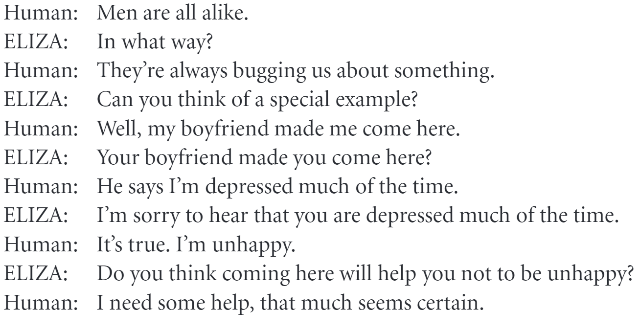
\includegraphics[width=.3\textwidth]{ELIZAExample.PNG}
\caption{\label{fig:eliza_example}An example of a conversation with ELIZA.}
\end{figure}

ELIZA used keyword mapping, where it searched the input for a word and associated rules with it. Like in the example, the keyword depressed triggers a response of “I’m sorry to hear that you are depressed”. While this may work well in certain instances, if the user was to ask a question, this technique would not work as well. To move away from these hard-coded responses you need to implement a type of machine learning environment. Machine learning will allow the program to learn new words or sentences without the need to hard-code these responses. An example of using a machine learning technique can be found in A.L.I.C.E., Artificial Linguistic Internet Computer Entity.

ALICE was created by Dr. Richard S. Wallace in 2003. While learning, ALICE creates an Artificial Intelligence Mark-Up Language which holds in general three different categories generated by a pattern consisting of words, spaces and wild-card symbols [2]. These categories are Atomic, Default and Recursive. A template is generated as a response for each category. The Atomic category holds all patterns that do not include the wild card, while the Default category holds all patterns that do have the wildcard symbols. Finally, the Recursive will hold categories that may be too large to accurately deduce a meaning, and hence need to be shortened into smaller ones. For example, “Hello *” would be categorized in the Default section and a templated response can be generated as “Hi there *”.

We will be using this type of categorizing with modification that these templated responses will be pulled from the Twitter API to emulate more real human responses. Using this technique will allow for reals-time categorization without the restriction of a permanent, static database. These responses will also reflect the currently used phrases and words. The idea is that while a more ridged response or “Template” may result in a higher acceptance rate from the user, a dynamically generated response will generate a more human like response that makes it less distinguishable as a computer program.

\section{Related Work}
Similar work with was done by Ritter et al. [3]. However, Ritter et al. focused more on the tagging of the Twitter conversations with the approach of unsupervised conversation models, where the discovery of acts amounts to clustering utterances with similar conversational roles. The goal of this was to eliminate the collection and tagging process and allow the learning algorithm to categorize how people converse in a new medium.

Banko and Etzioni instead attempted to use entire websites collected as a corpus for use with ALICE. At the beginning of each learning task, ALICE receives an unexplored concept $c(n)$ as input, instantiates the set of extraction patters (e.g such as ) with name of $c(n)$, (e.g. fruit such as ), applies them over the input corpus, and uses the assessment model to add high-probability instances of $c(n)$ to it’s theory [4]. This is beneficial in the fact that it was almost 80\% accurate but is not representative of normal speech behavior.

\section{Implementation}
The overall strategy of our implementation can be summarized as follows. We begin by receiving a sentence from a user through a command line interface. This sentence is classified into one of the eight broad categories provided by Ritter et al. [3], namely: Status, Question to Followers, Reference Broadcast, Question, Reaction, Comment, Answer, Response. We accomplish this classification by utilizing the Pattern python library from Smedt and Daelemans [5] to perform parts of speech tagging. A probability of the sentence being in each category is assigned using these tagged parts of speech, and the sentence will be placed in the category with the highest probability. Meanwhile, we will also maintain a continuously updating local database of Twitter messages which will be classified according to the same eight categories stated above.

\begin{figure}[h]
\centering
\includegraphics[height=.4\textwidth]{chatbot_flowchart_logic.png}
\caption{\label{fig:chatbot_flowchart}Logic flowchart for our chatbot.}
\end{figure}

Our chatbot will then search through our local database for tweets in the category which best corresponds to being a good response to the user input sentence. For example, if the input sentence is classified as a Question, then the chatbot will search for tweets in the Answer category. Each result from the list of returned tweets will then be ranked by assigning a value representing the level of similarity to the input sentence. This value ranking will utilize a formula based on the total number of common noun (NN) keywords that are in the same narrow category in each tweet.

\begin{algorithm}[H]
RankResponse$(tweets)$
    \begin{algorithmic}[1]
    \State $R = []$\Comment{Initialize our list of responses}
    \For {each tweet in tweets}
        \State $r = $ NumCommonNouns(tweet, input)
        \State InsertSorted(r, tweet, R)
    \EndFor
    \State return $R[0]$\Comment{The top ranking result will be returned}
    \end{algorithmic}
\end{algorithm}

Examples of narrow categories are Italian Food, Video Games, or Computer Science. The chatbot will respond to the user input sentence with the highest ranked of these tweets in the database.

\section{Evaluation Methods}
We will evaluate the effectiveness of our chatbot both qualitatively and quantitatively. First, to evaluate our chatbot qualitatively, we will ask a specific question, and then determine whether the response from the chatbot seemed human-like. This evaluation method will obviously necessarily require a degree of subjectivity, but will nonetheless allow us to judge the relative effectiveness of the chatbot in holding a conversation.

Second, in order to quantitatively evaluate the effectiveness of our chatbot, we will adopt a method inspired by Ritter et al. [3]. This method will attempt to objectively rate the conversational accuracy of the chatbot in terms of its ability to replicate an actual twitter conversation. In other words, we will use a real tweet as input to the chatbot. Then, we will expect the response given by the chatbot to be the actual tweet given by a human in a real world conversation. We will rate the overall effectiveness of the chatbot by calculating the percentage of conversations it correctly predicted. We will consider our chatbot to be a success if it's percentage of correct conversation predictions is near 80\%.

\section{Future Explorations}
A key advantage to our chatbot approach is that it will more closely mimic real human conversations by including slang and other less formal language available in Twitter messages. However, an obvious downside to our approach is that using real verbatim tweets means that the chatbot's responses will be less personalized. For example, currently, our chatbot cannot refer to its conversation partner by a specific name unless, by coincidence, a real tweet happens to contain that name.

Therefore, a future area of exploration for our chatbot could include modifying its response so that it is not an exact verbatim tweet. For example, if we know that the chatbot is conversing with someone named Bob, we could inject that name in front of the tweet in specific contexts. In order to accomplish this, we would need to ensure that the name injection resulted in a coherent tweet. This would involve more closely analyzing the parts of speech of the response tweet in order to make accurate injections specific to the context of the conversation and sentence structure.

\section{References}
[1] Weizenbaum, J. (1966). ELIZA-A computer program for the study of natural language communication between man and machine. Communications of the ACM.\\

\noindent[2] Wallace, R. (2003). The elements of AIML style. ALICE AI Foundation.\\

\noindent[3] Ritter, A., Cherry, C., \& Dolan, B. (2010, June). Unsupervised modeling of twitter conversations. In \textit{Human Language Technologies: The 2010 Annual Conference of the North American Chapter of the Association for Computational Linguistics} (pp. 172-180). Association for Computational Linguistics.\\

\noindent[4] Banko M., Etzioni O., (2007). Strategies for Lifelong Knowledge Extraction from the Web. Turing Center, University of Washington.\\

\noindent[5] Smedt, T. D., \& Daelemans, W. (2012). Pattern for python. Journal of Machine Learning Research, 13(Jun), 2063-2067.

\end{document}
